\chapter{Explainability}
\label{ch_explainability}
%
During evaluation of the benchmark study, we found that proset models are very open to inspection after fitting.
This is due to their built-in feature selection and geometric structure.
In this chapter, we review diagnostic plots and other techniques that provide a better understanding of model behavior.
%
\section{Low-dimensional representations of the data}
\label{sec_low_dimensional}
%
Verification of the model structure is greatly simplified if the algorithm is able to reduce the inputs to a small set.
We can then conduct what amounts to post-fit exploratory data analysis.\par
%
In the benchmark study, the proset classifier achieves the largest reduction in the number of features for the cancer data set, where only 4 out of 30 features yield a model that is still equivalent to XGBoost in terms of log-loss (see Table \ref{tab_e3_e8_e9}).
With only four inputs, we can visually inspect all scatter plots involving a combination of two features.
Figure \ref{fig_scatter_plots_cancer} shows the positions of the prototypes (large circles) and test samples (small circles).
The three misclassified cases are circled in black.
The density plots on the diagonal show the marginal distributions for each feature, both for the prototypes (solid curves / vertical lines) and test samples (dashed curves / dots).
Two interesting findings are that (a) any pair of features allows us to distinguish the two classes fairly well and (b) the prototypes are more clearly separated with lower variance than the whole population.\par
%
\begin{figure}
\caption{Scatter plots for active features of the cancer data model}
\label{fig_scatter_plots_cancer}
%
\begin{center}
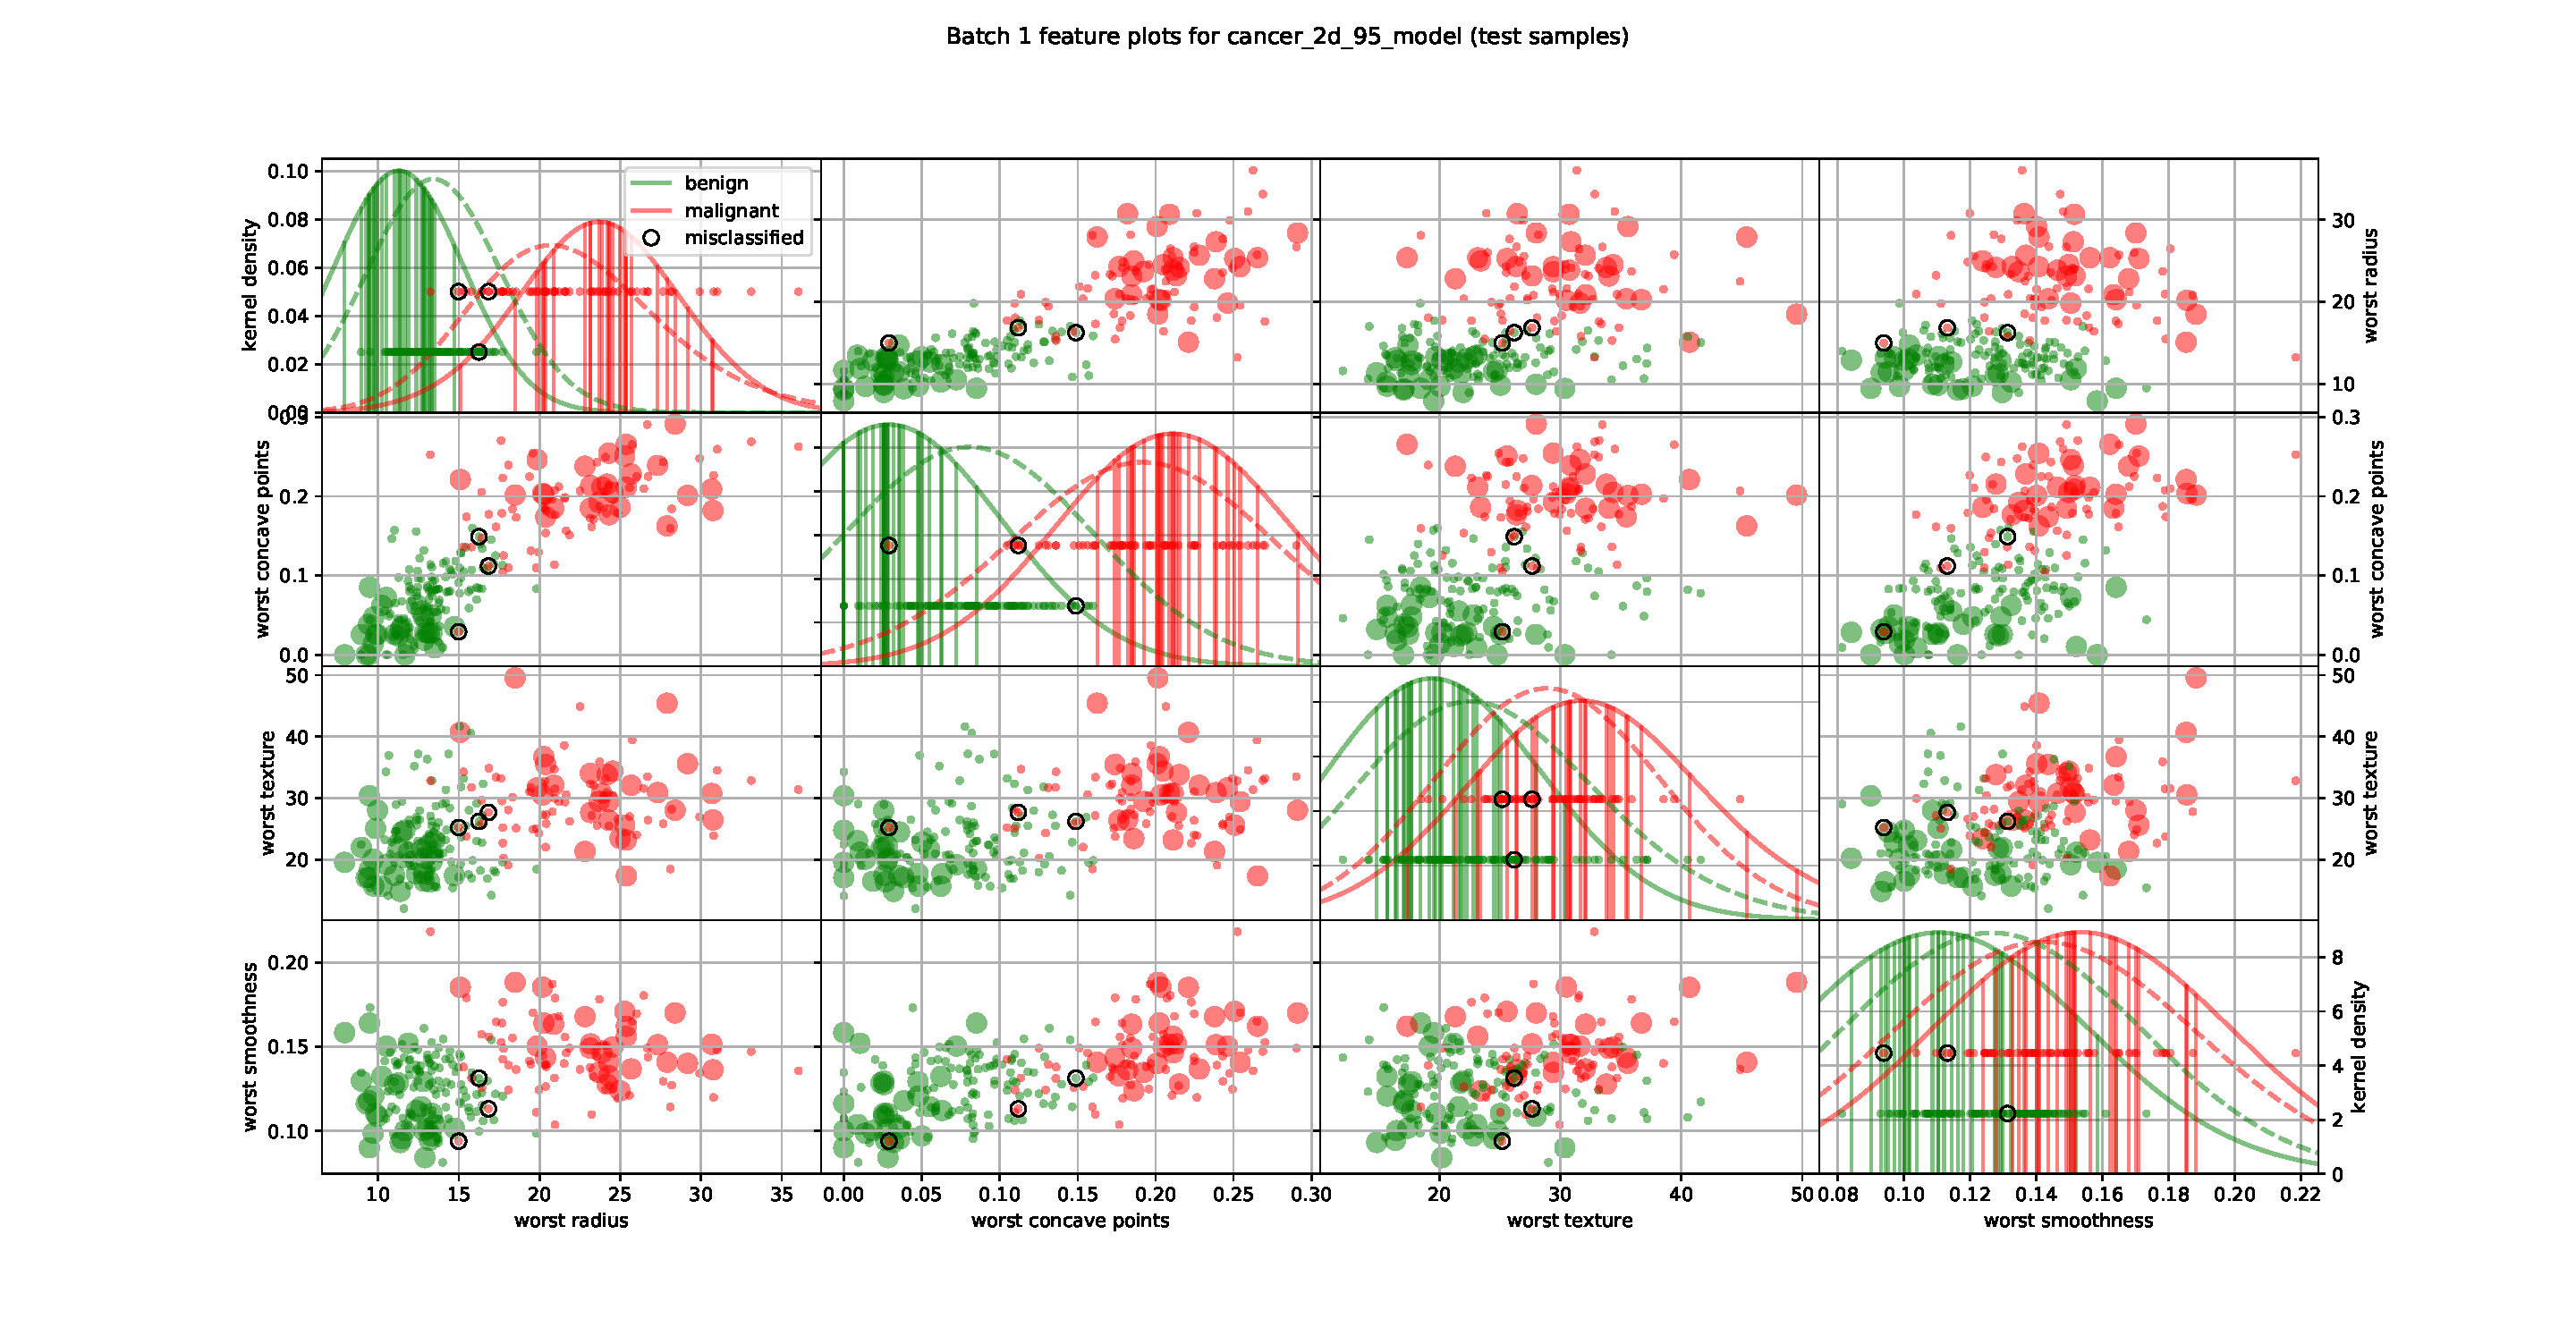
\includegraphics[width=0.95\textheight, angle=90]{figures/cancer_scatter_plot_testing_data.pdf}
\end{center}
\end{figure}
%
A `small' model is also easier to review for domain experts.
For example, an oncologist should be able to provide a clear assessment whether the four features (in decreasing order of weights: worst radius, worst concave points, worst texture, worst smoothness) are a natural and sufficient choice of indicators.
If we have access to the original image data, we can ask experts to review the misclassified cases in detail and compare them to the most similar prototypes.
This can reveal labeling errors, important features excluded by the algorithm due to dearth of relevant training samples, or genuine `hard cases' that are difficult to classify even for humans.\par
%
A technique that can work even if the number of features remains large is to create low-dimensional maps of the data that take model fit results into account.
For the visualization we call the `batch 1 map', we perform doubly weighted PCA on the prototypes of the first batch:\par
%
Let $Z\in\R^{J_1\times D}$ be the matrix obtained by rescaling the features for the prototypes of the first batch with the corresponding feature weights:
%
\begin{equation}
Z_{j,d}:=v_{1,d}x_{s_{1,j},d}\label{eq_scaled_x}
\end{equation}
%
This gives larger impact to features for which the algorithm is more sensitive and removes any deselected features from the analysis.
Now let $\overline{z}$ be the row mean of $Z$ weighted using the prototype weights:
%
\begin{equation}
\overline{z}:=\frac{\sum_{j=1}^{J_1}w_{1,j}Z_{j,\bullet}}
{\sum_{j=1}^{J_1}w_{1,j}}\label{eq_weighted_mean}
\end{equation}
%
Denote by $\overline{Z}$ the centered matrix
%
\begin{equation}
\overline{Z}_{j,d}:=Z_{j,d}-\overline{z}_d\label{eq_centered_Z}
\end{equation}
%
Let $W\in\R^{J_1\times J_1}$ be the diagonal matrix with diagonal elements $w_{1,j}$ and compute the matrix decomposition
%
\begin{equation}
\overline{Z}^TW\overline{Z}=:U\Sigma U^T\label{eq_weighted_svd}
\end{equation}
%
In the above, $\Sigma$ is the diagonal matrix of eigenvalues with row and column dimension equal to the rank of $\overline{Z}^TW\overline{Z}$, while $U$ is the corresponding orthogonal matrix of eigenvectors.
If $\Sigma$ has at least rank two, the `batch 1 map' coordinates for the prototypes of the first batch are the first two columns of the product $\overline{Z}U$.
Other samples can be mapped via the same transform, i.e., scale with $v_1$, center with $\overline{z}$, and multiply with $U$.\par
%
\begin{figure}
\caption{`Batch 1 map' of cancer data showing test samples}
\label{fig_batch_1_map_test}
%
\begin{center}
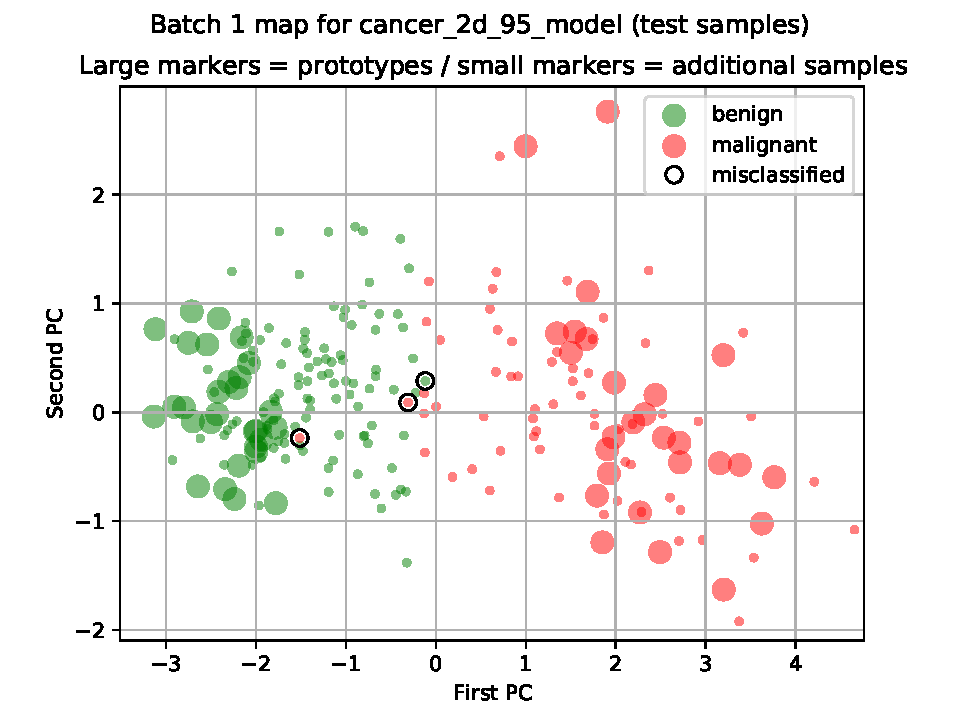
\includegraphics[height=0.4\textheight]{figures/cancer_batch_1_map_testing_data.pdf}
\end{center}
\end{figure}
%
The `batch 1 map' for the prototypes and test set of the cancer data is shown in Figure \ref{fig_batch_1_map_test}.
It appears that the two classes are almost linearly separable except for the three misclassified samples.
Two are close to the boundary between the classes, while the last is a `malignant' case surrounded by `benign' cases.
%
\section{Assessing the familiarity of new samples}
\label{sec_familiarity}
%
\begin{figure}
\caption{Model behavior outside the `area of competence'}
\label{fig_area_of_competence}
%
\begin{center}
\subfloat[\textbf{kNN on the rotated checkerboard}]{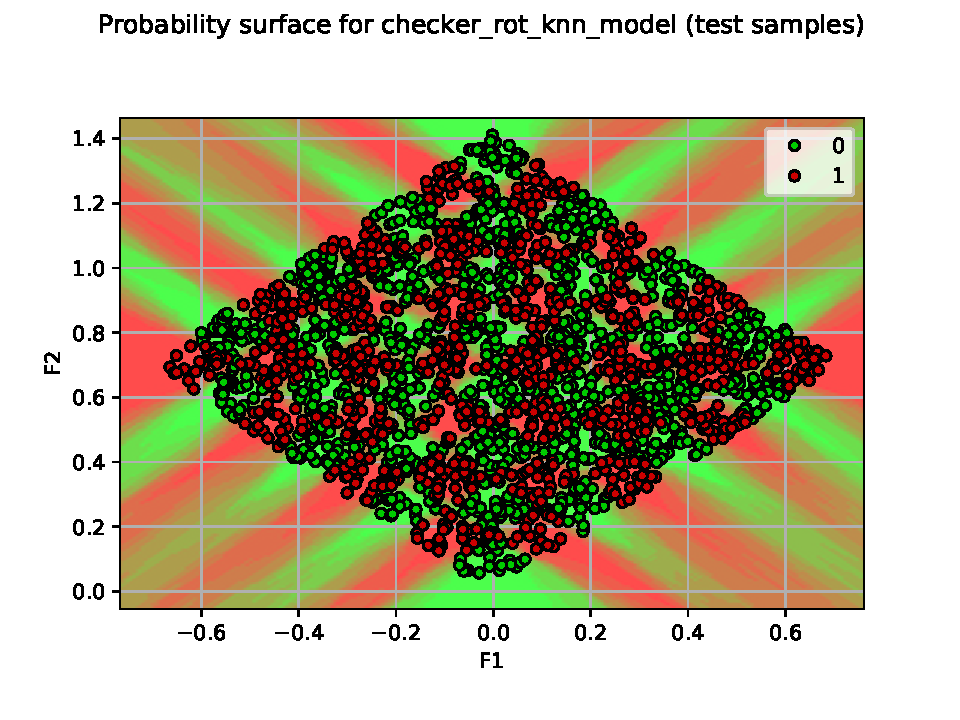
\includegraphics[width=0.49\textwidth]{figures/checker_rot_knn_surf_test.pdf}}
\subfloat[\textbf{XGBoost on the rotated checkerboard}]{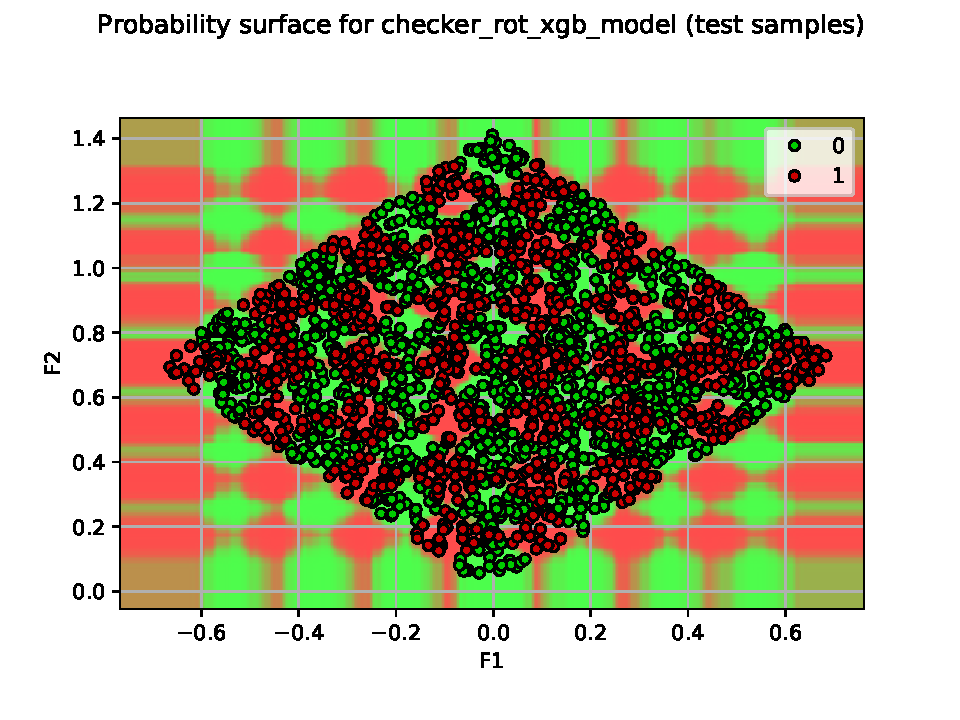
\includegraphics[width=0.49\textwidth]{figures/checker_rot_xgb_surf_test.pdf}}\\
\subfloat[\textbf{proset on the rotated checkerboard}]{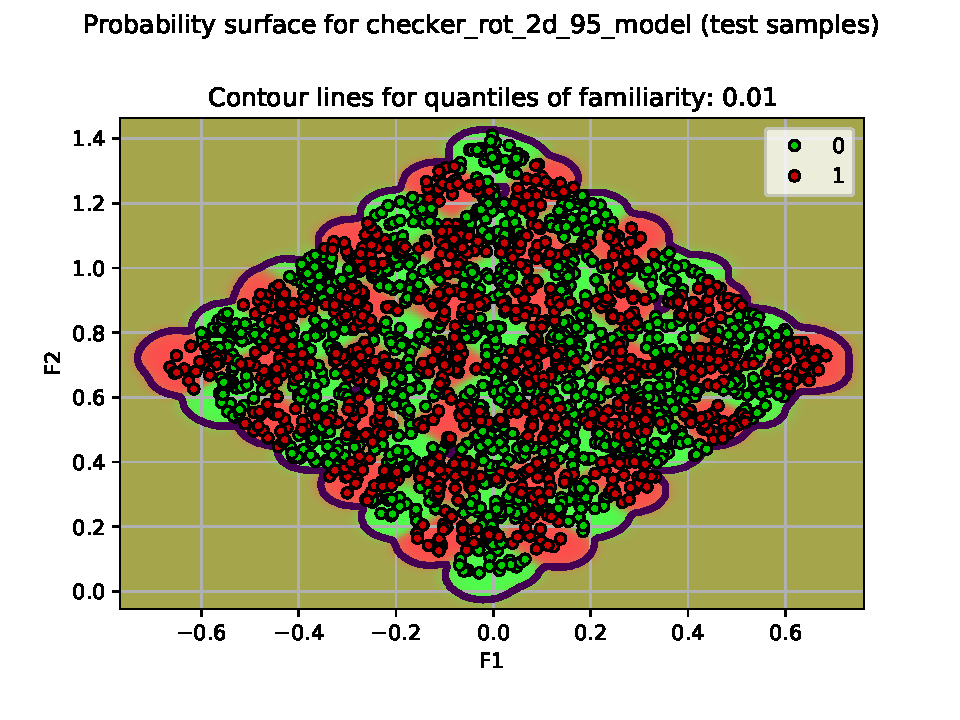
\includegraphics[width=0.49\textwidth]{figures/checker_rot_surf_test.pdf}}
\end{center}
\end{figure}
%
One problem faced by all machine learning is that their behavior becomes arbitrary for samples that are far removed from the original training data.
The way a model extrapolates outside its `area of competence' depends entirely on the specific algorithm and does not reflect any empirical evidence.
This is illustrated in Figure \ref{fig_area_of_competence} for the rotated checkerboard example.
The plots show the probability surfaces for each of the three classifiers studied in Chapter \ref{ch_classifier}, i.e., the color scale represents the estimated probability for class 1 from green (0.0) to red (1.0).
While kNN and XGBoost create idiosyncratic patterns in regions of the feature space with no training data, proset reverts to the marginal distribution.
The proset estimate is no more correct than that of the other two algorithms, but we consider it the most `honest' in the absence of information.
For balanced training data as in the example, proset does not assign a high probability to an arbitrary class as may happen with kNN or XGBoost.
Given that users tend to interpret the probability of the class with the highest probability estimate as the model's `confidence' in the result, this is an important advantage.\par
%
The proset algorithm can even provide an explicit indicator that a new sample is far away from the training data.
For any $x\in\R^D$, we define the familiarity of a proset model with $x$ as
%
\begin{equation}
\mathfrak{f}(x):=\sum_{b=1}^B\sum_{j=1}^{J_b}w_{b,j}G_{v_b}(x-x_{s_{b,j}})\label{eq_familiarity}
\end{equation}
%
This is just the denominator of (\ref{eq_pkx}) minus 1, which can be provided alongside the estimate with no additional effort.
Familiarity measures the total contribution of the weighted prototypes to the estimate relative to the marginal distribution represented by the 1.\par
%
Instead of using the absolute size of $\mathfrak{f}(x)$ to assess new samples, we find it more useful to express it as a quantile of the distribution of familiarity observed for test data.
As the model may overfit its training data slightly, it is better to use held-out data for this analysis.
Figure \ref{fig_area_of_competence} shows the resulting 1 \% contour line of familiarity for the proset classifier.
For a new sample, familiarity expressed as a quantile of the previously observed distribution can be interpreted as p-value of a statistical test whether the estimate is inside the model's `area of competence'.\par
%
For a supervised learning problem with many features, the training data is typically close to a `thin' manifold in the high-dimensional feature space.
Using quantiles of familiarity as indicated above, we can measure proximity to that manifold via a scalar indicator.
This is a powerful tool for monitoring a machine learning model in production and to detect data drift.
However, there is a trade-off between feature selection and the usefulness of familiarity.
Consider the case where proset does not select a feature because of insufficient variation in the training data.
A new sample that has a markedly different value in that one feature is still assigned a high familiarity score if the features actually used by the model lie in the expected range.
%
\section{Explaining individual estimates}
\label{sec_individual_explanations}
%
\subsection{Explanation report}
\label{sec_explanation_report}
%
\begin{figure}
\caption{Example of explanation report for cancer data}
\label{fig_explanation_report}
%
\begin{center}
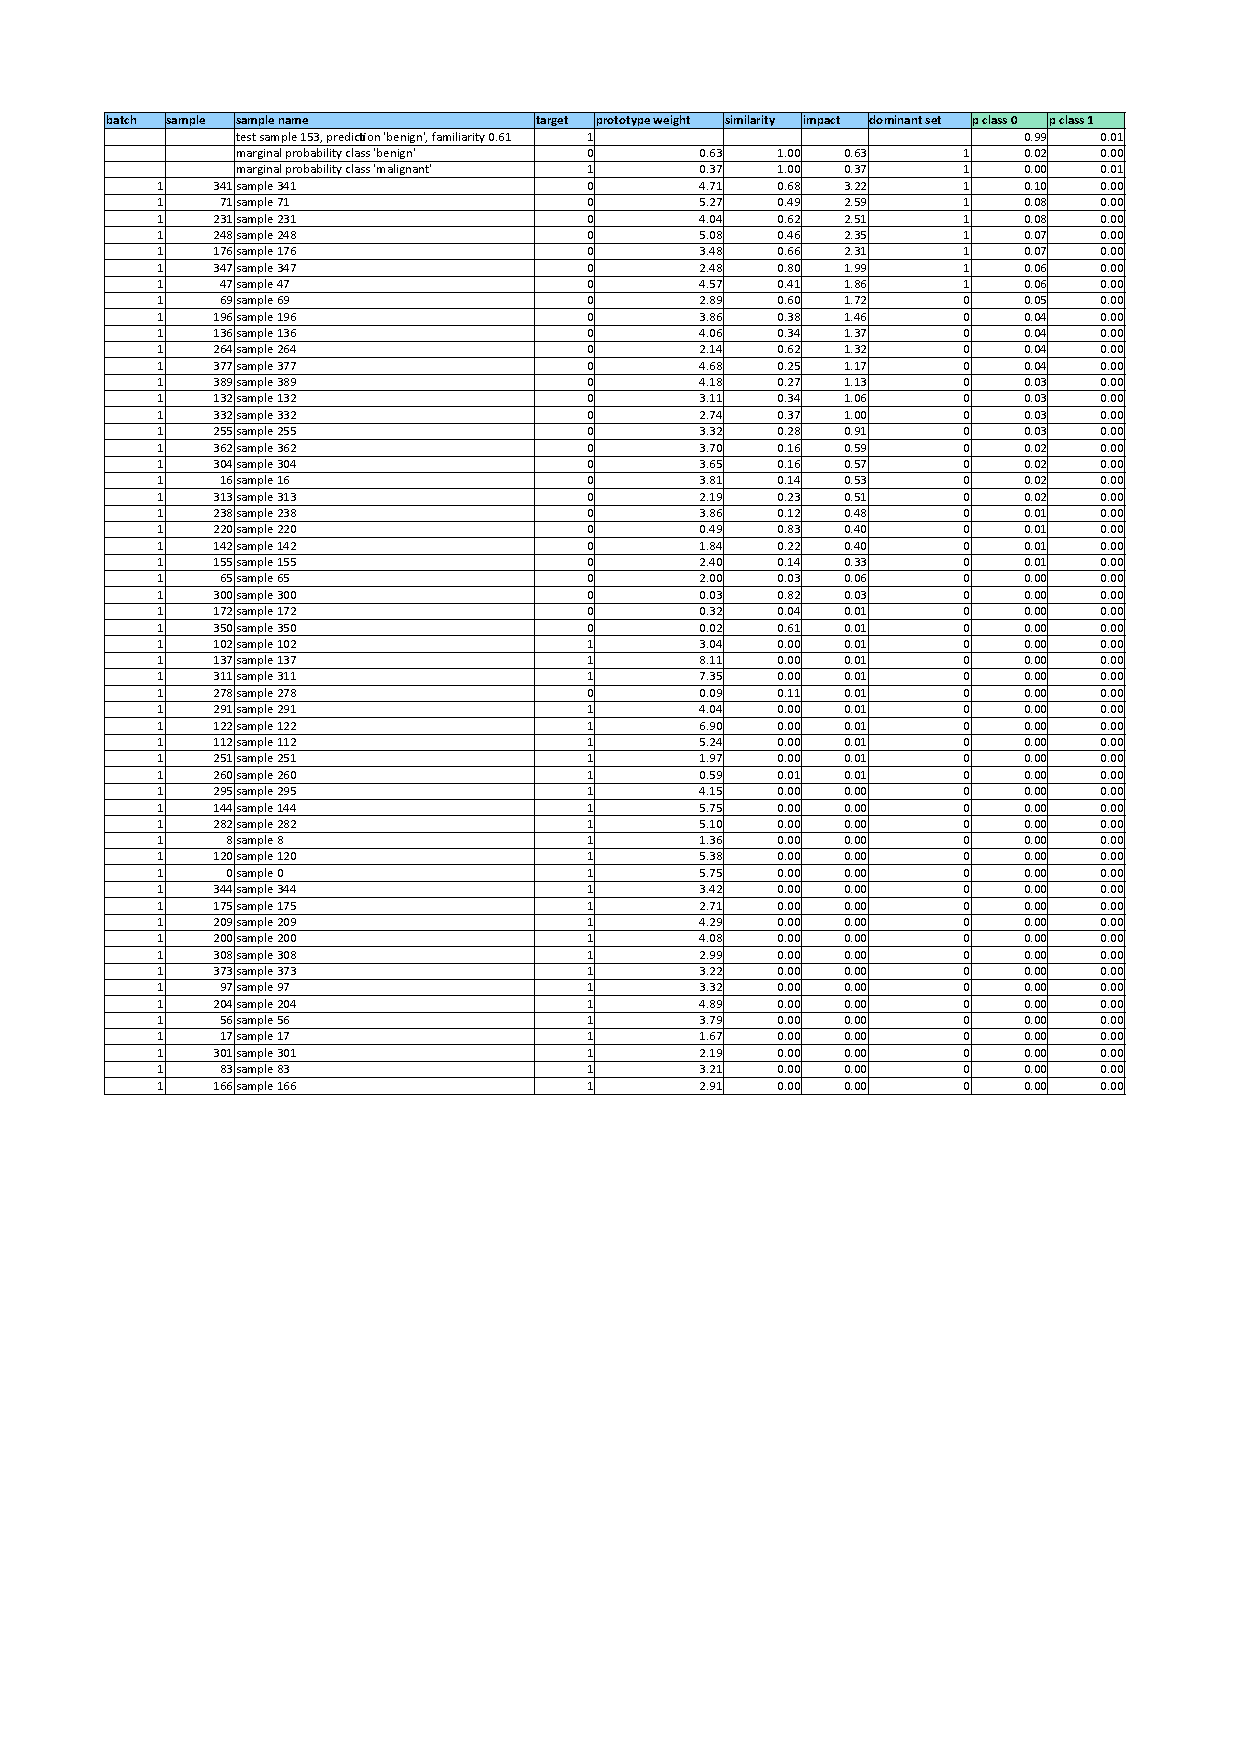
\includegraphics[width=0.99\textwidth]{figures/cancer_2d_95_model_explain.pdf}
\end{center}
\end{figure}
%
Our implementation of proset can export information about the model as tabular data.
The basic report contains information on all prototypes, their weights, and active features.
A more interesting report relates a particular sample to the selected prototypes.
Figure \ref{fig_explanation_report} shows an example analysis for the proset classifier.
It deals with the one misclassified `malignant' case from the cancer data example that is surrounded by `benign' cases.
The report contains the following information:
%
\begin{description}
\item[Batch:] the number of the batch to which each prototype belongs.
The model in the example has only a single batch.
The first three rows contain information on the misclassified sample and the marginal distribution, they are not associated with any batch.
%
\item[Sample:] the zero-based index of the prototype with respect to the ordering of the training data after the train-test split.
%
\item[Sample name:] the record for the test sample states its zero-based index within the set of test data, the class with the highest estimated probability, and familiarity expressed as a quantile of the distribution for the test data.
The remaining rows indicate whether they belong to the marginal distribution or individual prototypes.
%
\item[Target:] the numeric representation of the class, either 0 (`benign') or 1 (`malignant').
The first rows contains the true target for the test sample.
%
\item[Prototype weight:] the value $w_{b,j}$ for each prototype.
The test sample has no entry, records for the marginal distribution show the marginal probability for the corresponding class.
%
\item[Similarity:] the value of the unnormalized Kernel $G_{v_b}$ at $x-x_{s_{b,j}}$.
This is a number in $(0,1]$, where $1$ indicates that the sample features $x$ are identical to those of the prototype.
The test sample has no entry, records for the marginal probabilities list a 1 as they affect all estimates equally.
%
\item[Impact:] the product of prototype weight and similarity is the total impact of the prototype on the estimated probability (\ref{eq_pkx}).
By default, the report lists the prototypes in order of descending impact.
%
\item[Dominant set:] a binary indicator of observations that have the largest impact on the estimate.
The target values for prototypes outside the dominant set can be changed without affecting which class is assigned the highest probability.
See below for a precise definition of the dominant set.
%
\item[p class 0:] the record for the test sample shows the estimated probability for class 0 (`benign').
The remaining rows contain the additive contribution of the marginal distribution and prototypes to this estimate.
The contribution is equal to the impact listed for the row divided by the total impact if the target is 0.
Otherwise, the contribution is zero.
%
\item[p class 1:] as above for class 1 (`malignant').
\end{description}
%
The report provides a complete breakdown of the estimate for one sample into the contribution of the marginals and prototypes.
The multivariate structure of the feature space is replaced by a simple list that can be filtered and sorted by different criteria to identify major contributors.
While the total number of prototypes can be much larger than in the example, most tend to have negligible impact on any particular case.\par
%
For the computation of the `dominant set' indicator, we use the following procedure:
%
\begin{algorithm}[Dominant set]~
\label{alg_dominant_set}
%
\begin{enumerate}
\item Sort the prototypes in descending order of impact and assign a rank to each.
Prototypes with the same impact receive the same rank.
%
\item For each rank $r$, compute $p_{r,k}$ as sum of additive contributions (columns `p class 0', etc.\ in the report) to the probability estimate for class $k$ from the marginal distribution and prototypes up to rank $r$.
These satisfy $0<\sum_{k=0}^{K_1}p_{r,k}\leq 1$.
The remainder $t_r:=1-\sum_{k=0}^{K-1}p_{r,k}$ is the total contribution of prototypes with rank greater than $r$.
%
\item For each rank $r$, denote by $k_{1,r}$ and $k_{2,r}$ the classes with the largest and second largest value of $p_{r,k}$.
Determine the set  $R:=\{r:p_{r,k_{1_r}}-p_{r,k_{2,r}}>t_r\}$.
%
\item If $R$ is empty, the dominant set is empty.
Otherwise, all prototypes with a rank less than or equal to the minimal element in $R$ form the dominant set.
\end{enumerate}
\end{algorithm}
%
\begin{remark}
By constructions, if $R$ is not empty, it contains all ranks greater than or equal to its minimal element and all share the same value for $k_{1,r}$.
Thus, it contains all ranks where the remainder $t_r$ is too small to affect which class is assigned the highest probability.
\end{remark}
%
In the example report, the prototypes of the dominant set together with the marginal distribution contribute 53 percentage points of the 99 \% probability estimated for class 0.
Thus, class 0 would be assigned the highest probability even if all remaining prototypes belonged to class 1.
The purpose of the dominant set is to serve as a guideline which prototypes need to be reviewed for a better understanding of a particular result.\par
%
\begin{figure}
\caption{`Batch 1 map' of cancer data showing prototype impact}
\label{fig_batch_1_map_impact}
%
\begin{center}
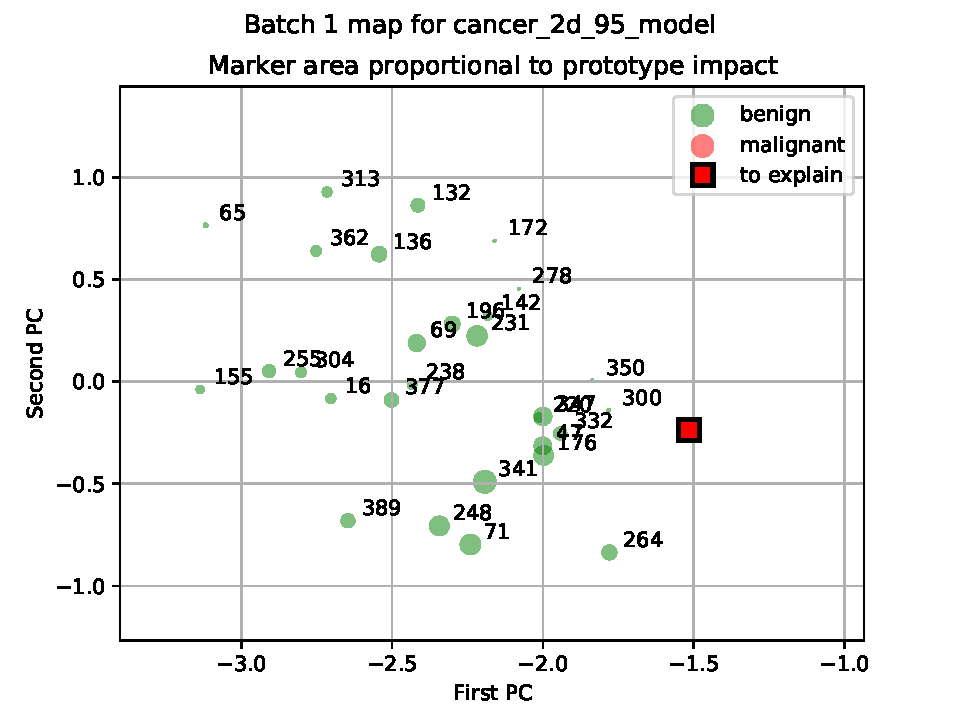
\includegraphics[height=0.4\textheight]{figures/cancer_batch_1_map_impact.pdf}
\end{center}
\end{figure}
%
The impact of prototypes on a particular estimate can also be visualized in the `batch 1 map'.
Figure \ref{fig_batch_1_map_impact} does this for the case from the example report.
The size of each circle is proportional to the impact of the prototype, numbers refer to the sample index.
%
\subsection{Combining SHAP values and geometric analysis}
\label{sec_shap_values}
%
So far, we have looked at model-specific explanations for proset estimators on their own.
In this section, we combine them with a model-agnostic approach to gain additional insight into the model structure.
We choose the SHAP (SHapley Additive exPlanations) method for assessing feature importance proposed by Lundberg and Lee \cite{Lundberg_17}.
SHAP provides explanations for individual estimates and is the only additive feature attribution method that has certain desirable properties.
A downside is that the computational effort grows exponentially in the number of features, although an efficient algorithm exists for decision trees \cite{Lundberg_18}.
To facilitate usage of SHAP, our implementation of proset allows `shrinking' the model to take only the features with nonzero weights as input.\par
%
SHAP explains an estimate by comparing the sample of interest to a reference point.
The relative change in the estimator between the points is attributed to the relative change in the features.
There appears to be little research so far on the best choice of reference point, but Izzo et.\ al.\ \cite{Izzo_20} consider the issue.
The authors point out that the common choice of using the origin of the feature space as baseline is not satisfactory.
For a binary classifier, they recommend to select a reference point on the decision boundary between the two classes.
They refer to this as a `neutral baseline', since the algorithm is indifferent which class to choose.
We cannot follow this approach, as we want to study the probability estimate itself without reference to a decision rule\footnote{
We do use the `naive' decision rule that selects the class with the highest estimated probability to define bins for Algorithm \ref{alg_bins} and to compute balanced accuracy as a secondary metric for the benchmark study.
See the discussion in the next paragraph why we do not consider this rule for further analysis.
}.
Also, several of the benchmark cases have more than two classes and it is not certain that a point can be found that is `neutral' with regards to all of them at once.\par
%
We believe that classification should always be carried out in two stages by combining a stochastic model with a decision rule.
The purpose of the former is to accurately estimate the probability distribution with no regard to the practical problem we want to solve.
The purpose of the latter is to optimize the expected value of a problem-specific utility or loss function under the estimated distribution.
Any algorithm that conflates the two stages implicitly applies an arbitrary decision rule that is likely to yield sub-optimal results.
As an example, consider a credit scoring algorithm that estimates the default probability for loans.
It is doubtful that the lending company wants to grant loans to all applicants with default probability less than 50 \%.
A more thorough discussion of this issue can be found, e.g., in a blog article by Harrell \cite{Harrell_20}.\par
%
For the above reason, we want to find a suitable reference point for explaining the estimated probabilities themselves regardless of any decision rule that could be applied later.
We expect such a point to have the following three properties:
%
\begin{enumerate}
\item The point itself represents a feasible combination of features.
%
\item The point is not extreme in terms of the feature space.
For every feature, there are training samples that have either a higher or lower value.
%
\item The point is not extreme in terms of the estimated probabilities.
For every class, there are training samples that have either a higher or lower estimate.
\end{enumerate}
%
\begin{remark}
\begin{enumerate}
\item Property 1 acknowledges that the baseline is part of the explanation and should have no `unnatural' characteristics.
There is less risk of misinterpreting the feature importance if they are computed with respect to a relatable feature vector.
%
\item Properties 2 and 3 mean that SHAP can explore changes of the input and output in all directions.
%
\item Property 3 can be viewed as a weaker notion of the `neutral baseline' proposed in \cite{Izzo_20}.
%
\item Properties 1 and 2 are mutually exclusive for binary features.
Here, we prefer property 1, i.e., the baseline should be a genuine case and not a hypothetical half-way point.
\end{enumerate}
\end{remark}
%
One way to satisfy the first condition is to use an actually observed point as reference.
The first two conditions imply that a medoid\footnote{
A medoid is any point from a set for which the average absolute distances to all other points is minimal.
In one dimension, a medoid is also a median of the data.
} of the feature vectors for the training data is a suitable choice.
Likewise, condition 1 and 3 suggest to use a point whose estimated probabilities are a medoid of the probability vectors for the training data.
We thus propose the following procedure for choosing a baseline:
%
\begin{algorithm}[SHAP baseline]~
\label{alg_shap_baseline}
%
\begin{enumerate}
\item Rank all training samples in increasing order of average absolute distance to all other training samples in the feature space.
Use only features selected by proset to compute distances.
%
\item Rank all training samples in increasing order of average absolute distance to all other training samples in the space of estimated probability vectors.
%
\item Combine both rankings using Borda's rule\footnote{
Borda's rule converts rankings to scores by assigning each candidate half a point for each other candidate ranked the same, plus a full point for each candidate ranked worse.
Scores are totaled across rankings and the winners are the candidates with the most points.
} and use the winner as reference.
In case of a tie, choose the candidate whose probability vector has the highest entropy.
If still tied, use the point with the lowest sample index.
\end{enumerate}
\end{algorithm}
%
\begin{remark}
\begin{enumerate}
\item We do not recommend to combine the active features and estimated probabilities into a single vector.
The medoid property depends on the scaling of of individual variables and there is no obvious common scale.
Also, if there are many more features than classes, the former might dominate the decision.
Computing two separate rankings and using Borda's rule results in a choice that balances properties 2 and 3.
%
\item The method requires computing pairwise distances for all training samples, which may be unattractive for large problems.
In this case, we recommend subsampling.
\end{enumerate}
\end{remark}
%
\begin{figure}
\caption{`Batch 1 map' of cancer data showing reference point}
\label{fig_batch_1_map_reference}
%
\begin{center}
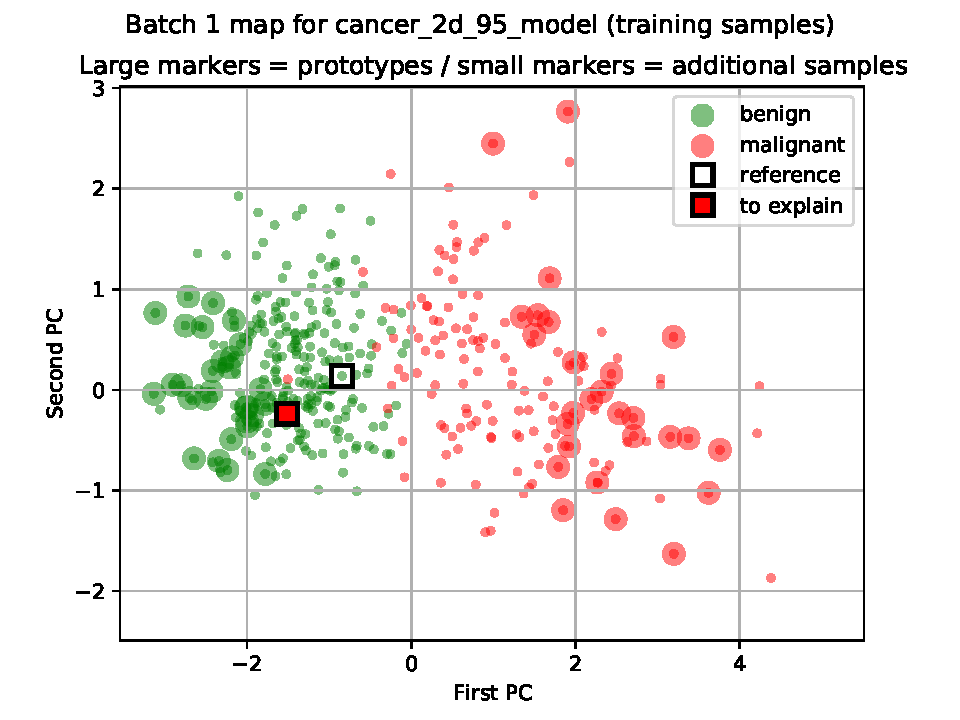
\includegraphics[height=0.4\textheight]{figures/cancer_batch_1_map_training_data_reference.pdf}
\end{center}
\end{figure}
%
\begin{figure}
\caption{SHAP feature importance}
\label{fig_feature_importance}
%
\begin{center}
\subfloat[\textbf{Global importance}]{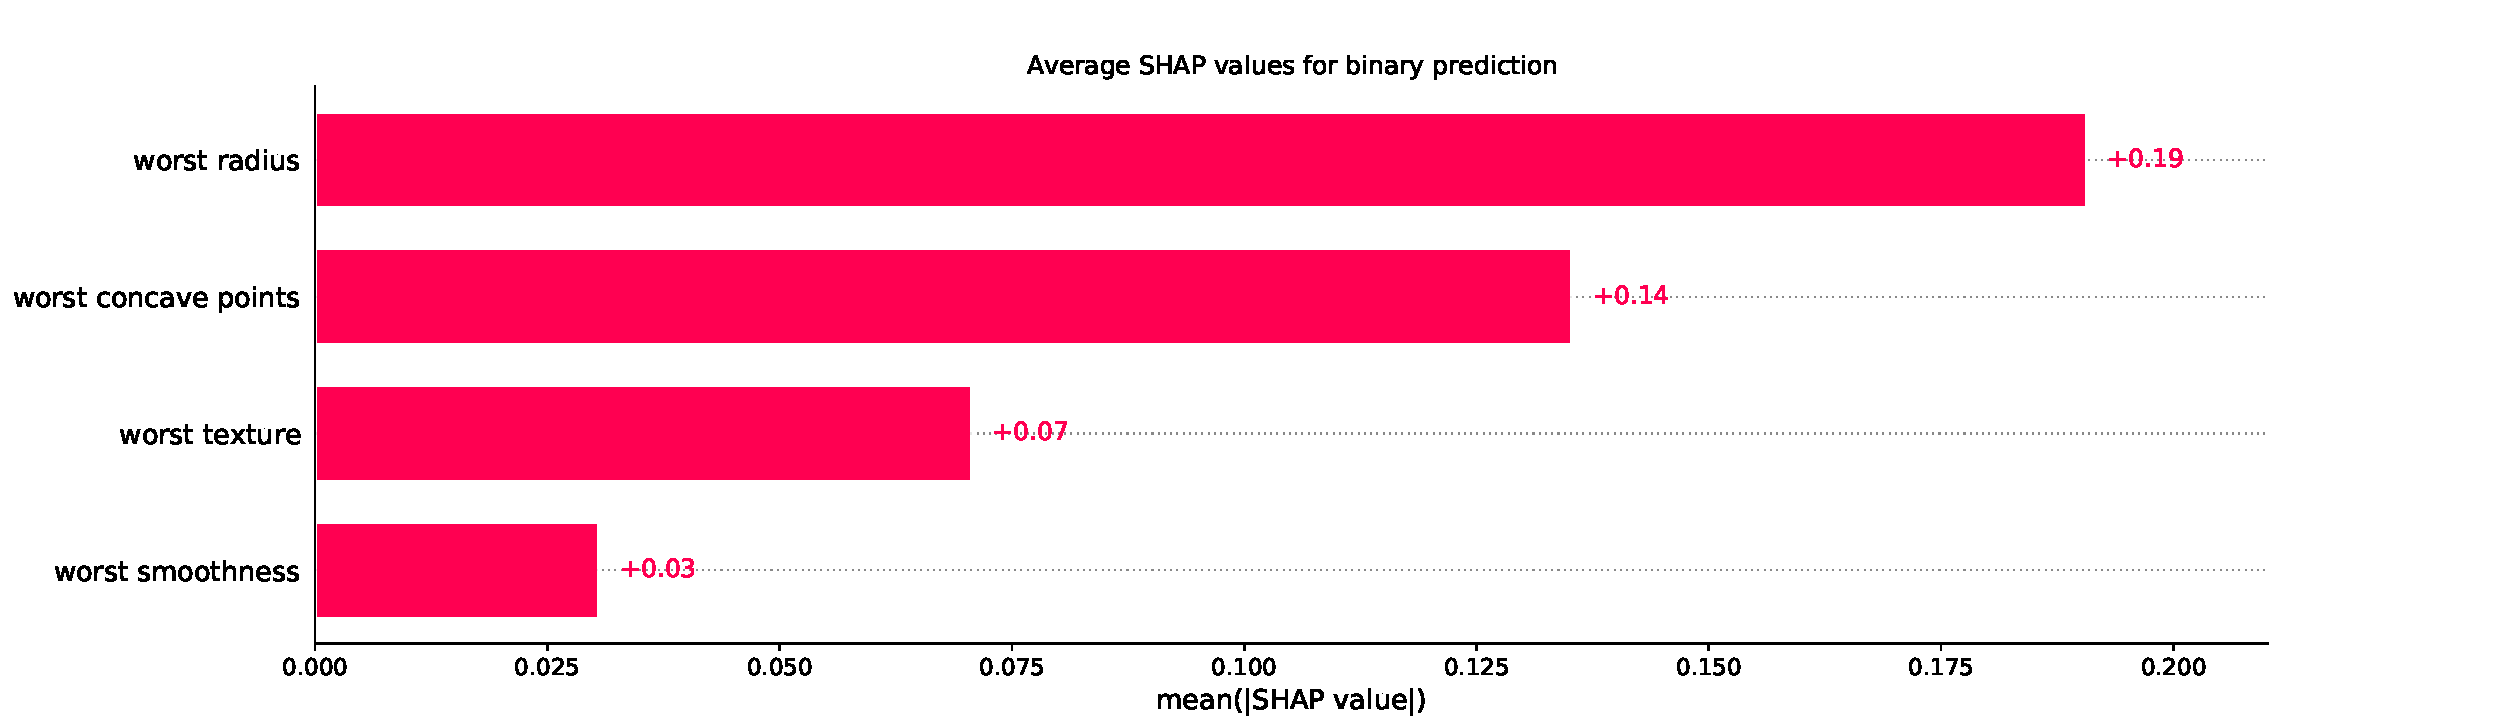
\includegraphics[width=0.99\textwidth]{figures/cancer_global_shap.pdf}}\\
\subfloat[\textbf{Misclassified case}]{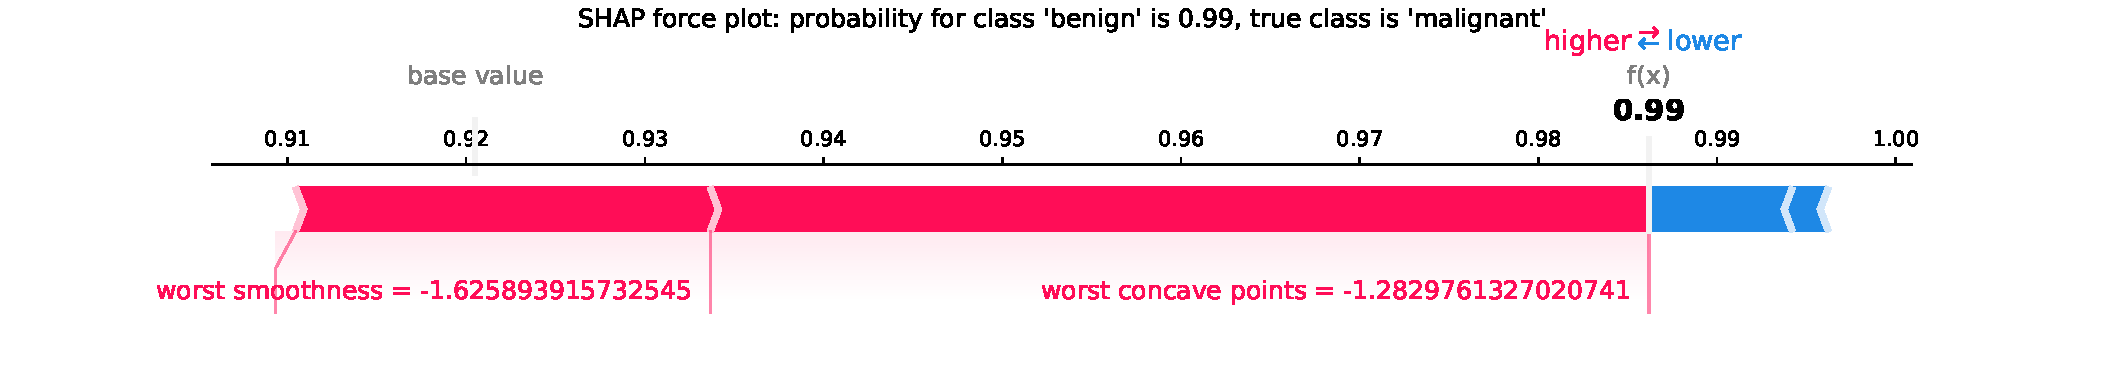
\includegraphics[width=0.99\textwidth]{figures/cancer_example_shap.pdf}}
\end{center}
\end{figure}
%
\begin{figure}
\caption{Scatter plots for important features}
\label{fig_scatter_important}
%
\begin{center}
\subfloat[\textbf{Global importance}]{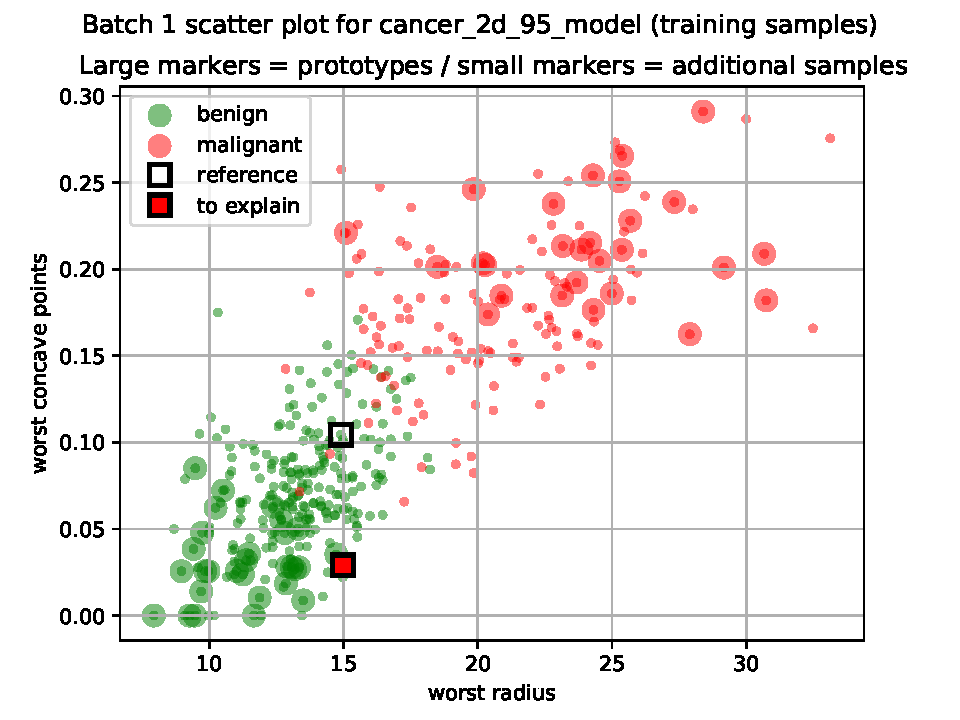
\includegraphics[height=0.4\textheight]{figures/cancer_scatter_global_shap.pdf}}\\
\subfloat[\textbf{Misclassified case}]{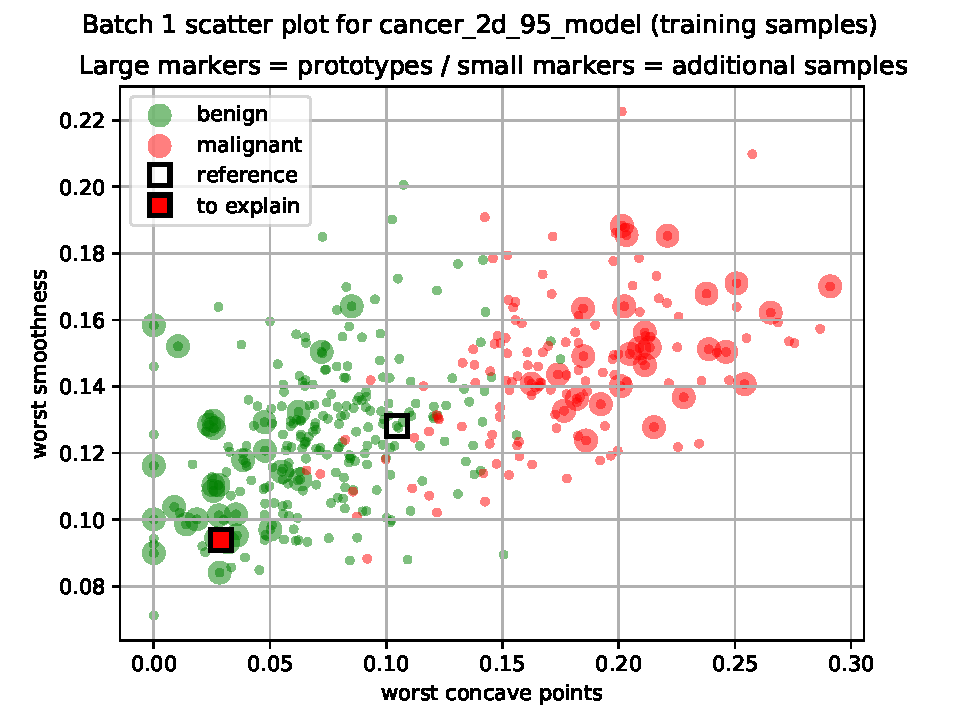
\includegraphics[height=0.4\textheight]{figures/cancer_scatter_example_shap.pdf}}
\end{center}
\end{figure}
%
\begin{figure}
\caption{Probability surfaces for important features}
\label{fig_probability_important}
%
\begin{center}
\subfloat[\textbf{Global importance}]{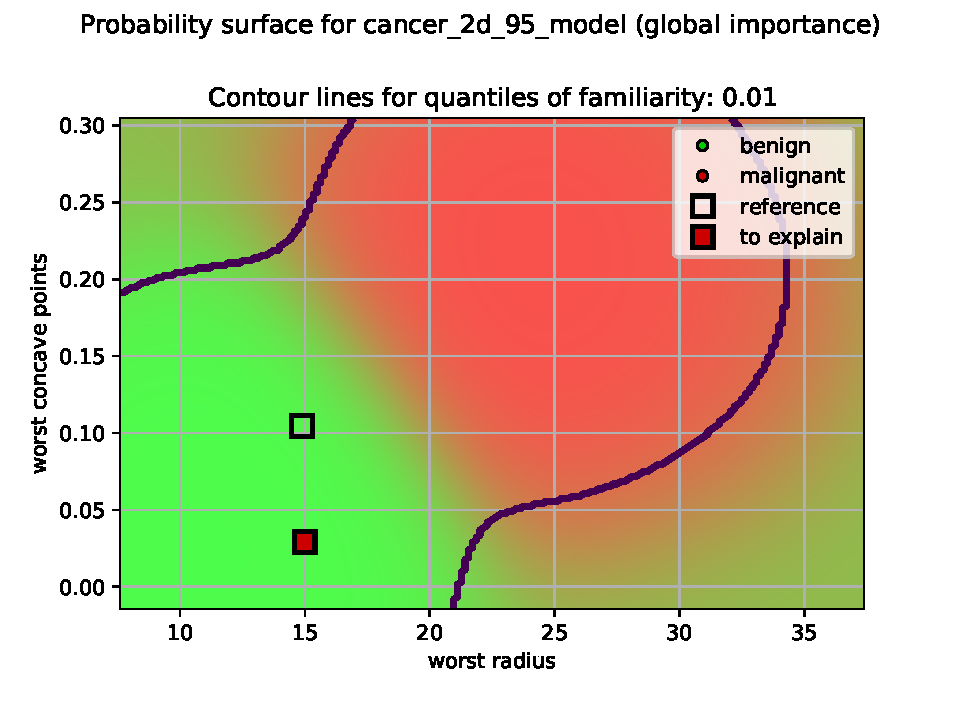
\includegraphics[height=0.4\textheight]{figures/cancer_surface_global_shap.pdf}}\\
\subfloat[\textbf{Misclassified case}]{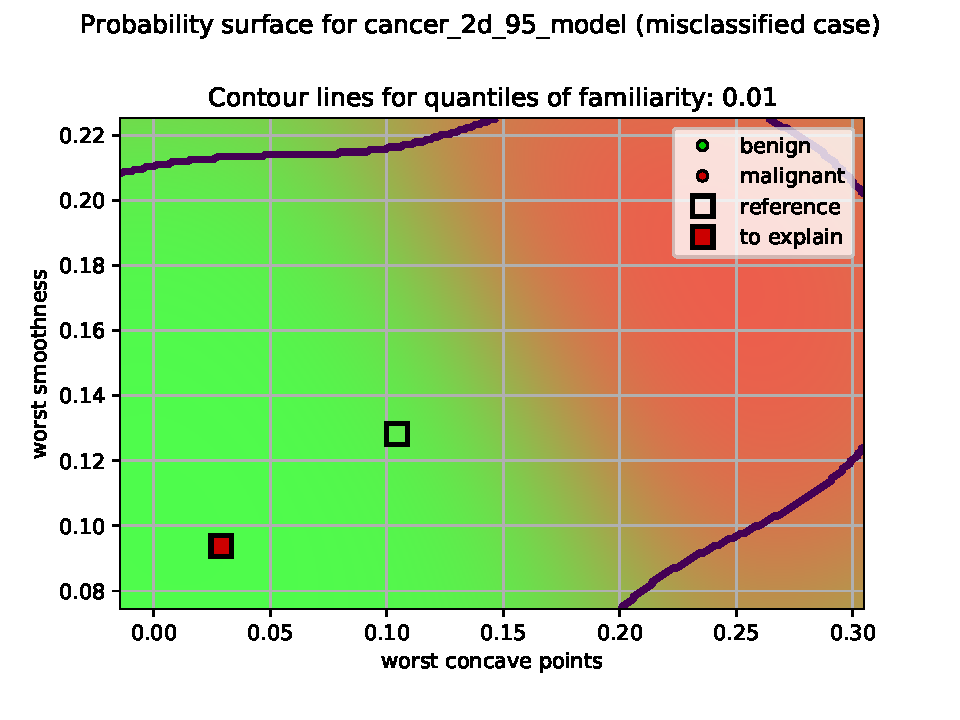
\includegraphics[height=0.4\textheight]{figures/cancer_surface_example_shap.pdf}}
\end{center}
\end{figure}
%
If we apply the above rule to the cancer data, it selects a baseline near the center of the point cloud of training samples.
The estimated probability for being `benign' is 92 \%, which is far from the 50 \% that would be achievable given the structure of the data.
However, the data is unbalanced in favor of `benign' cases and we have seen for the misclassified case in the previous section that probabilities in excess of 92 \% are achievable.
Figure \ref{fig_batch_1_map_reference} shows the reference point in a `batch 1 map' together with training data and the misclassified case we want to explain.\par
%
Figure \ref{fig_feature_importance} shows the results of SHAP analysis for the whole test data and the misclassified case.
Note that the global values are just the averages of the absolute scores of each feature across all samples.
Ordering the features by descending global importance yields the same sequence as for the feature weights, but we do not believe that this necessarily holds for every data set.
The two most important features globally are `worst radius' and `worst concave points'.
For the misclassified case, the estimate for class `benign' is shifted from 92 \% (baseline) to 99 \% because of the extremely low values for `worst concave points' and `worst smoothness'.
Figure \ref{fig_scatter_important} shows the bivariate scatter plots for both pairs of features, this time with training data as supplementary information.
As an alternative, we can study the probability surface resulting for the most important features if the other features are fixed at their values for the misclassified case.
This is shown in Figure \ref{fig_probability_important}.\par
%
\clearpage
%
\begin{figure}
\caption{`Batch 1 map' for digits data showing test samples}
\label{fig_batch_1_map_test_digits}
%
\begin{center}
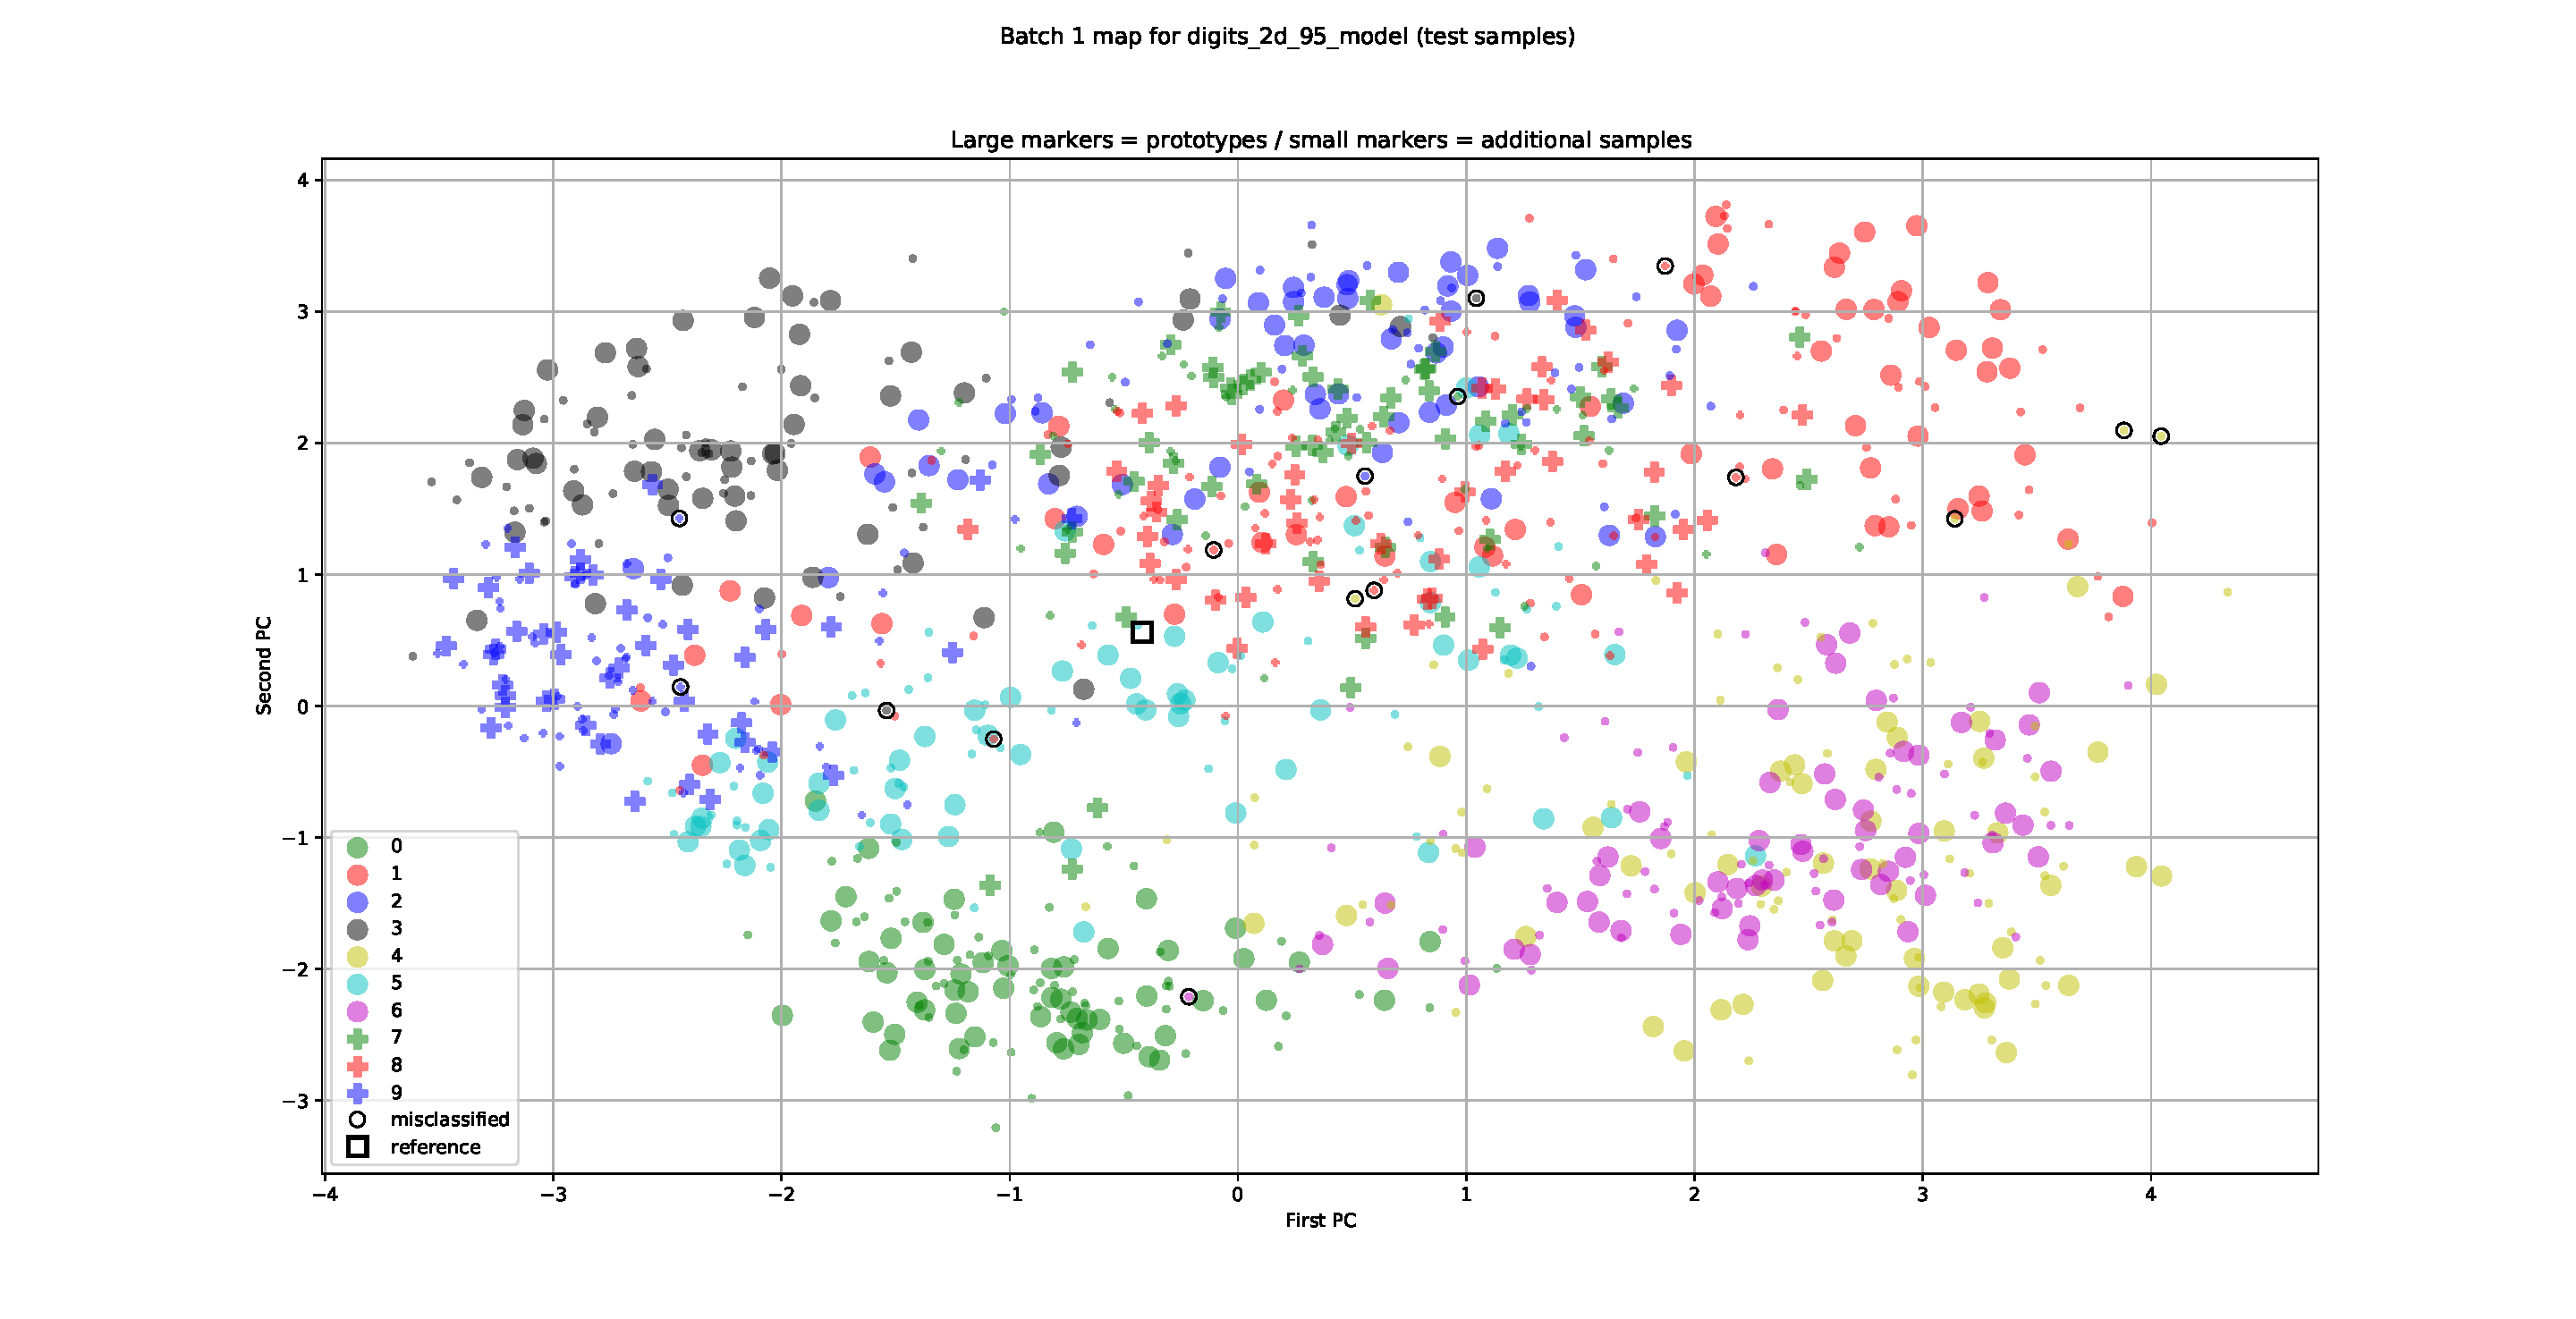
\includegraphics[width=0.95\textheight, angle=90]{figures/digits_batch_1_map.pdf}
\end{center}
\end{figure}
%
\begin{figure}
\caption{Explanation combining prototypes and SHAP values}
\label{fig_impact_shap}
%
\begin{center}
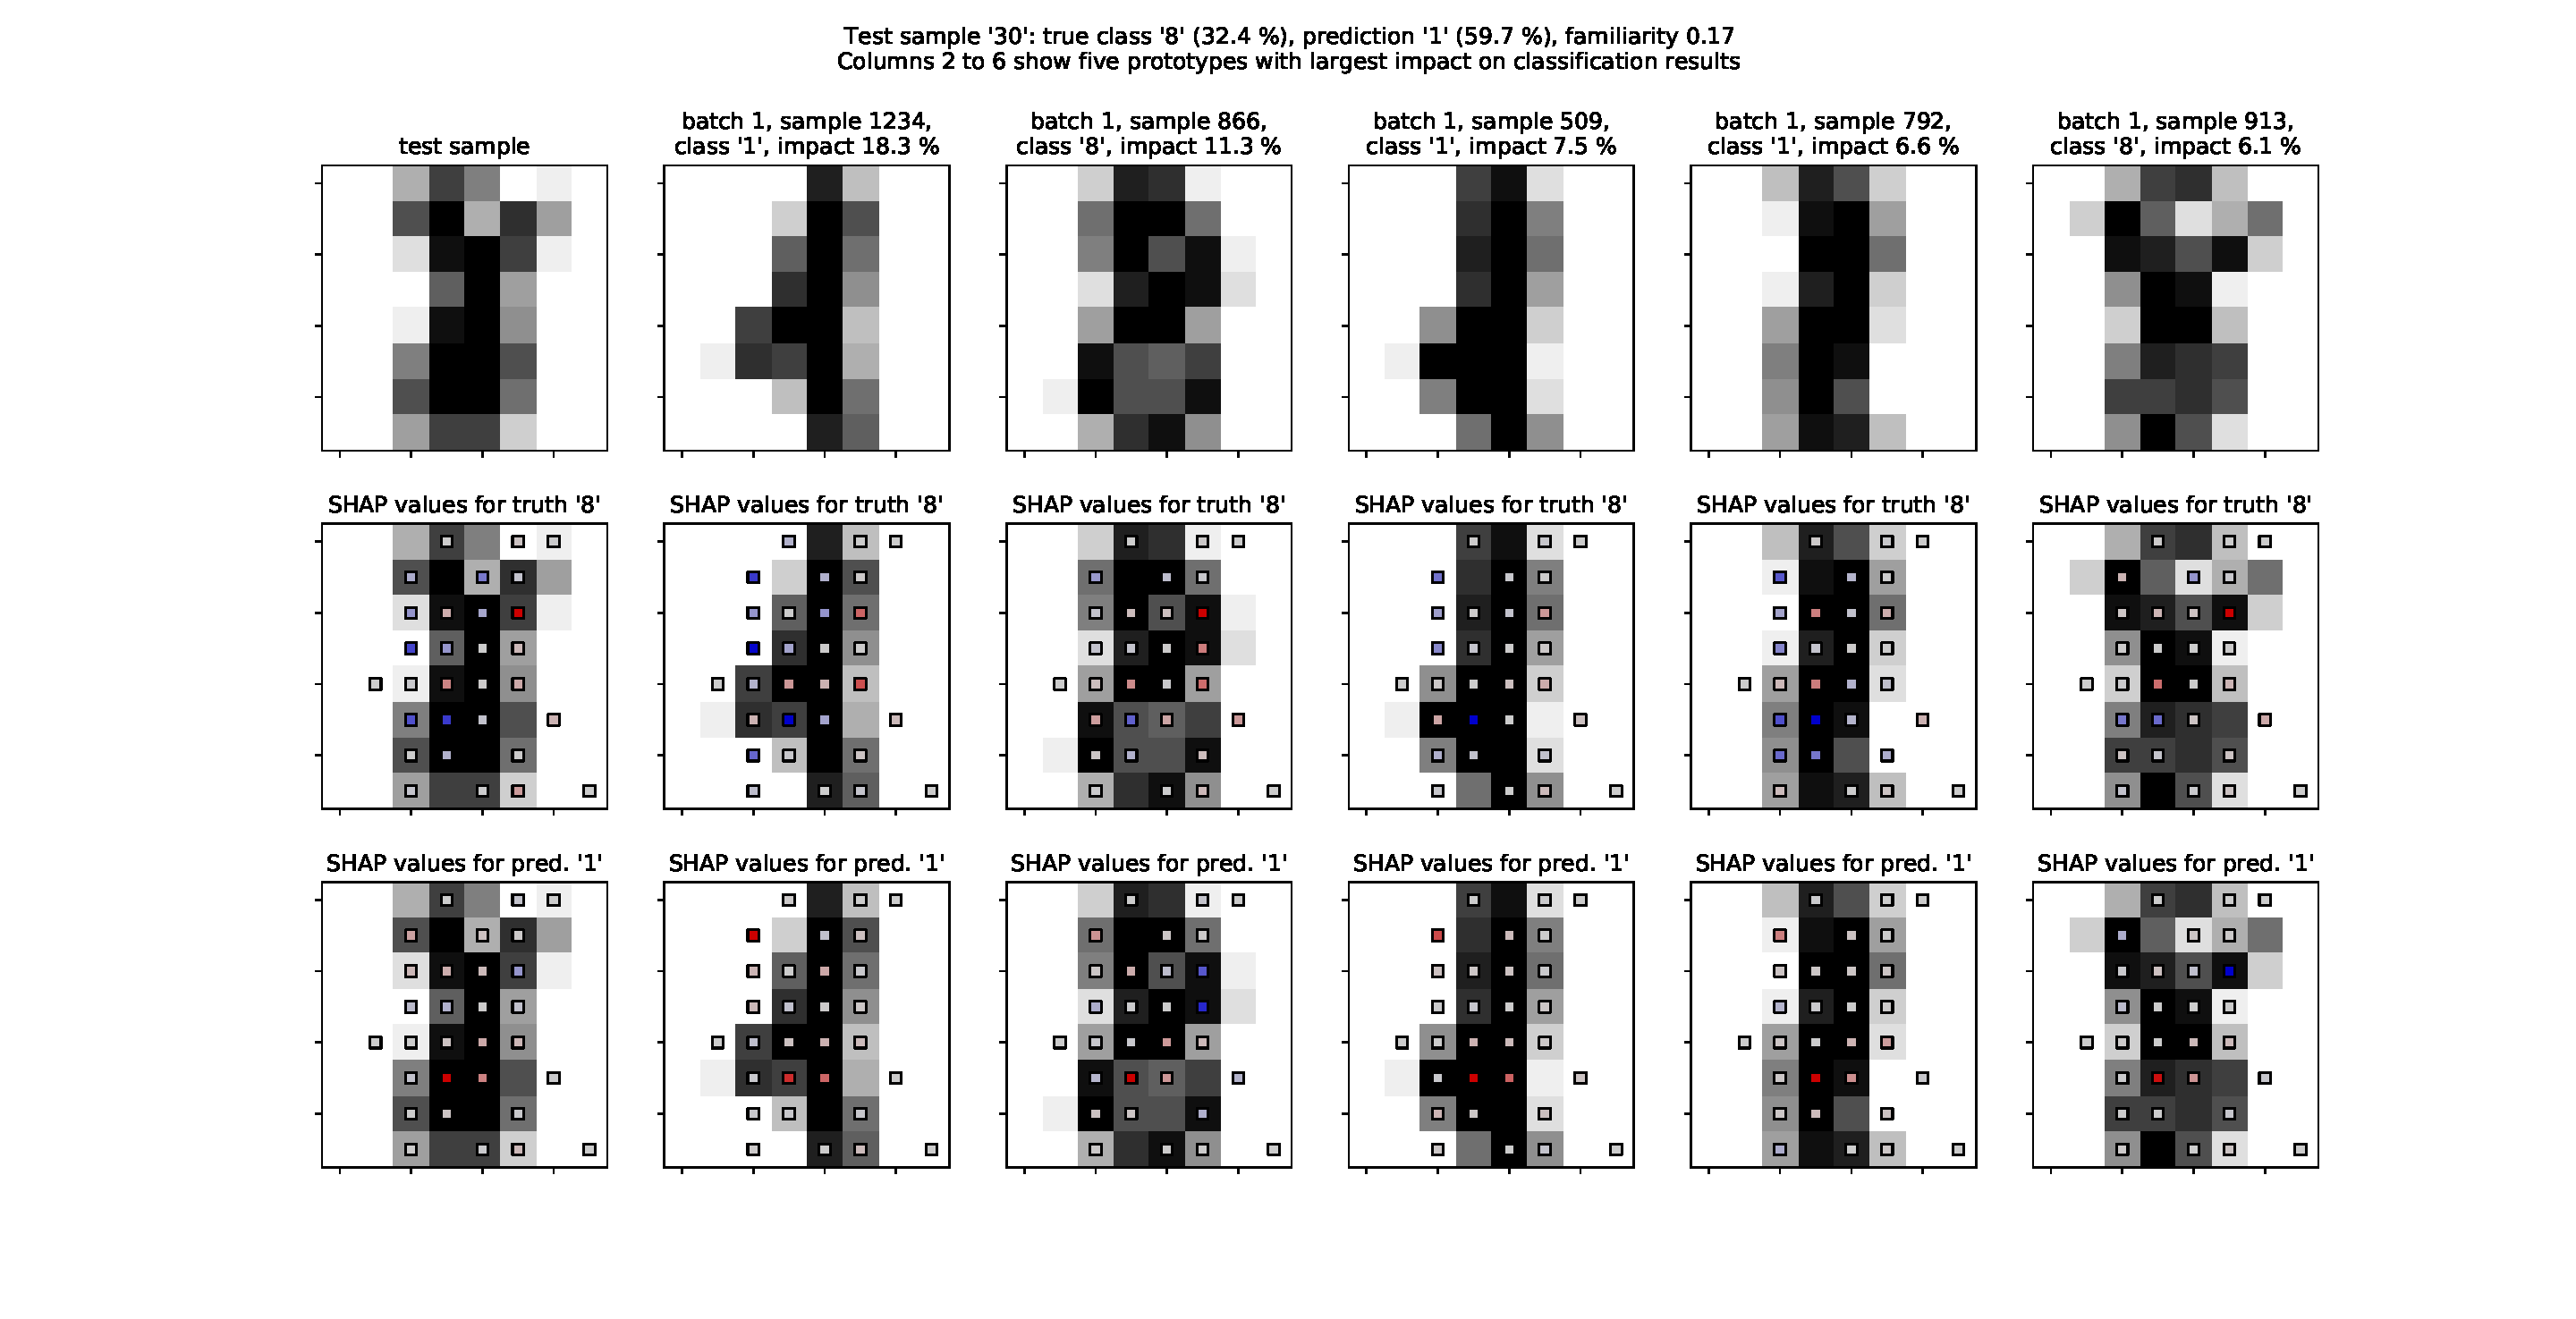
\includegraphics[width=0.95\textheight, angle=90]{figures/digits_8_vs_1_explanation.pdf}
\end{center}
\end{figure}
%
As a final example, we show how to create an explanation for the digits data set that relies both on prototypes with high impact and SHAP values.
This classification problem is more complex than the one for cancer data.
Figure \ref{fig_batch_1_map_test_digits} presents the `batch 1 map' including test data and a reference point selected using the ranking rule.
Several classes are well differentiated in this plot, but a two-dimensional representation clearly cannot capture the whole structure.\par
%
Figure \ref{fig_impact_shap} is a custom plot for explaining a particular misclassified digit.
It shows the case itself -- an `8' for which the highest probability is estimated for class `1' -- as well as the five prototypes with the largest impact on the result.
The second row overlays the SHAP values for the probability estimate of the true class `8', the third does the same for class `1'.
A red color indicates that the estimate is increased because of the grayscale value of the associated pixel, a blue color that it is decreased.
Note that the estimated probabilities for the baseline are 61 \% for class `8', 27 \% for class `3', and negligible for the other digits.
Thus, the SHAP values indicate the importance of the features for a shift away from this distribution towards 60 \% for class `1' and 32 \% for class `8'.
%
\endinput
